\section{问题构建}
\subsection{非线性运动学}
本文针对规避者$A$规避和目标到达场景，考虑在目标T附近部署两枚NCV ${D_1}$, ${D_2}$对规避者实施协同逼近。为表述简洁，后文除特殊说明外，统一定义下标$i \in \{ 1,2\} $，其中$i = 1$对应NCV ${D_1}$，$i = 2$对应NCV ${D_2}$。

规避者-目标-NCV 1-NCV 2四体相对运动关系如下图~\ref{fig:fourbody}所示，坐标系OXYZ为以目标T为原点、X轴位于水平面、Y轴竖直向上的地面坐标系。

\begin{figure}[!ht]
\centering
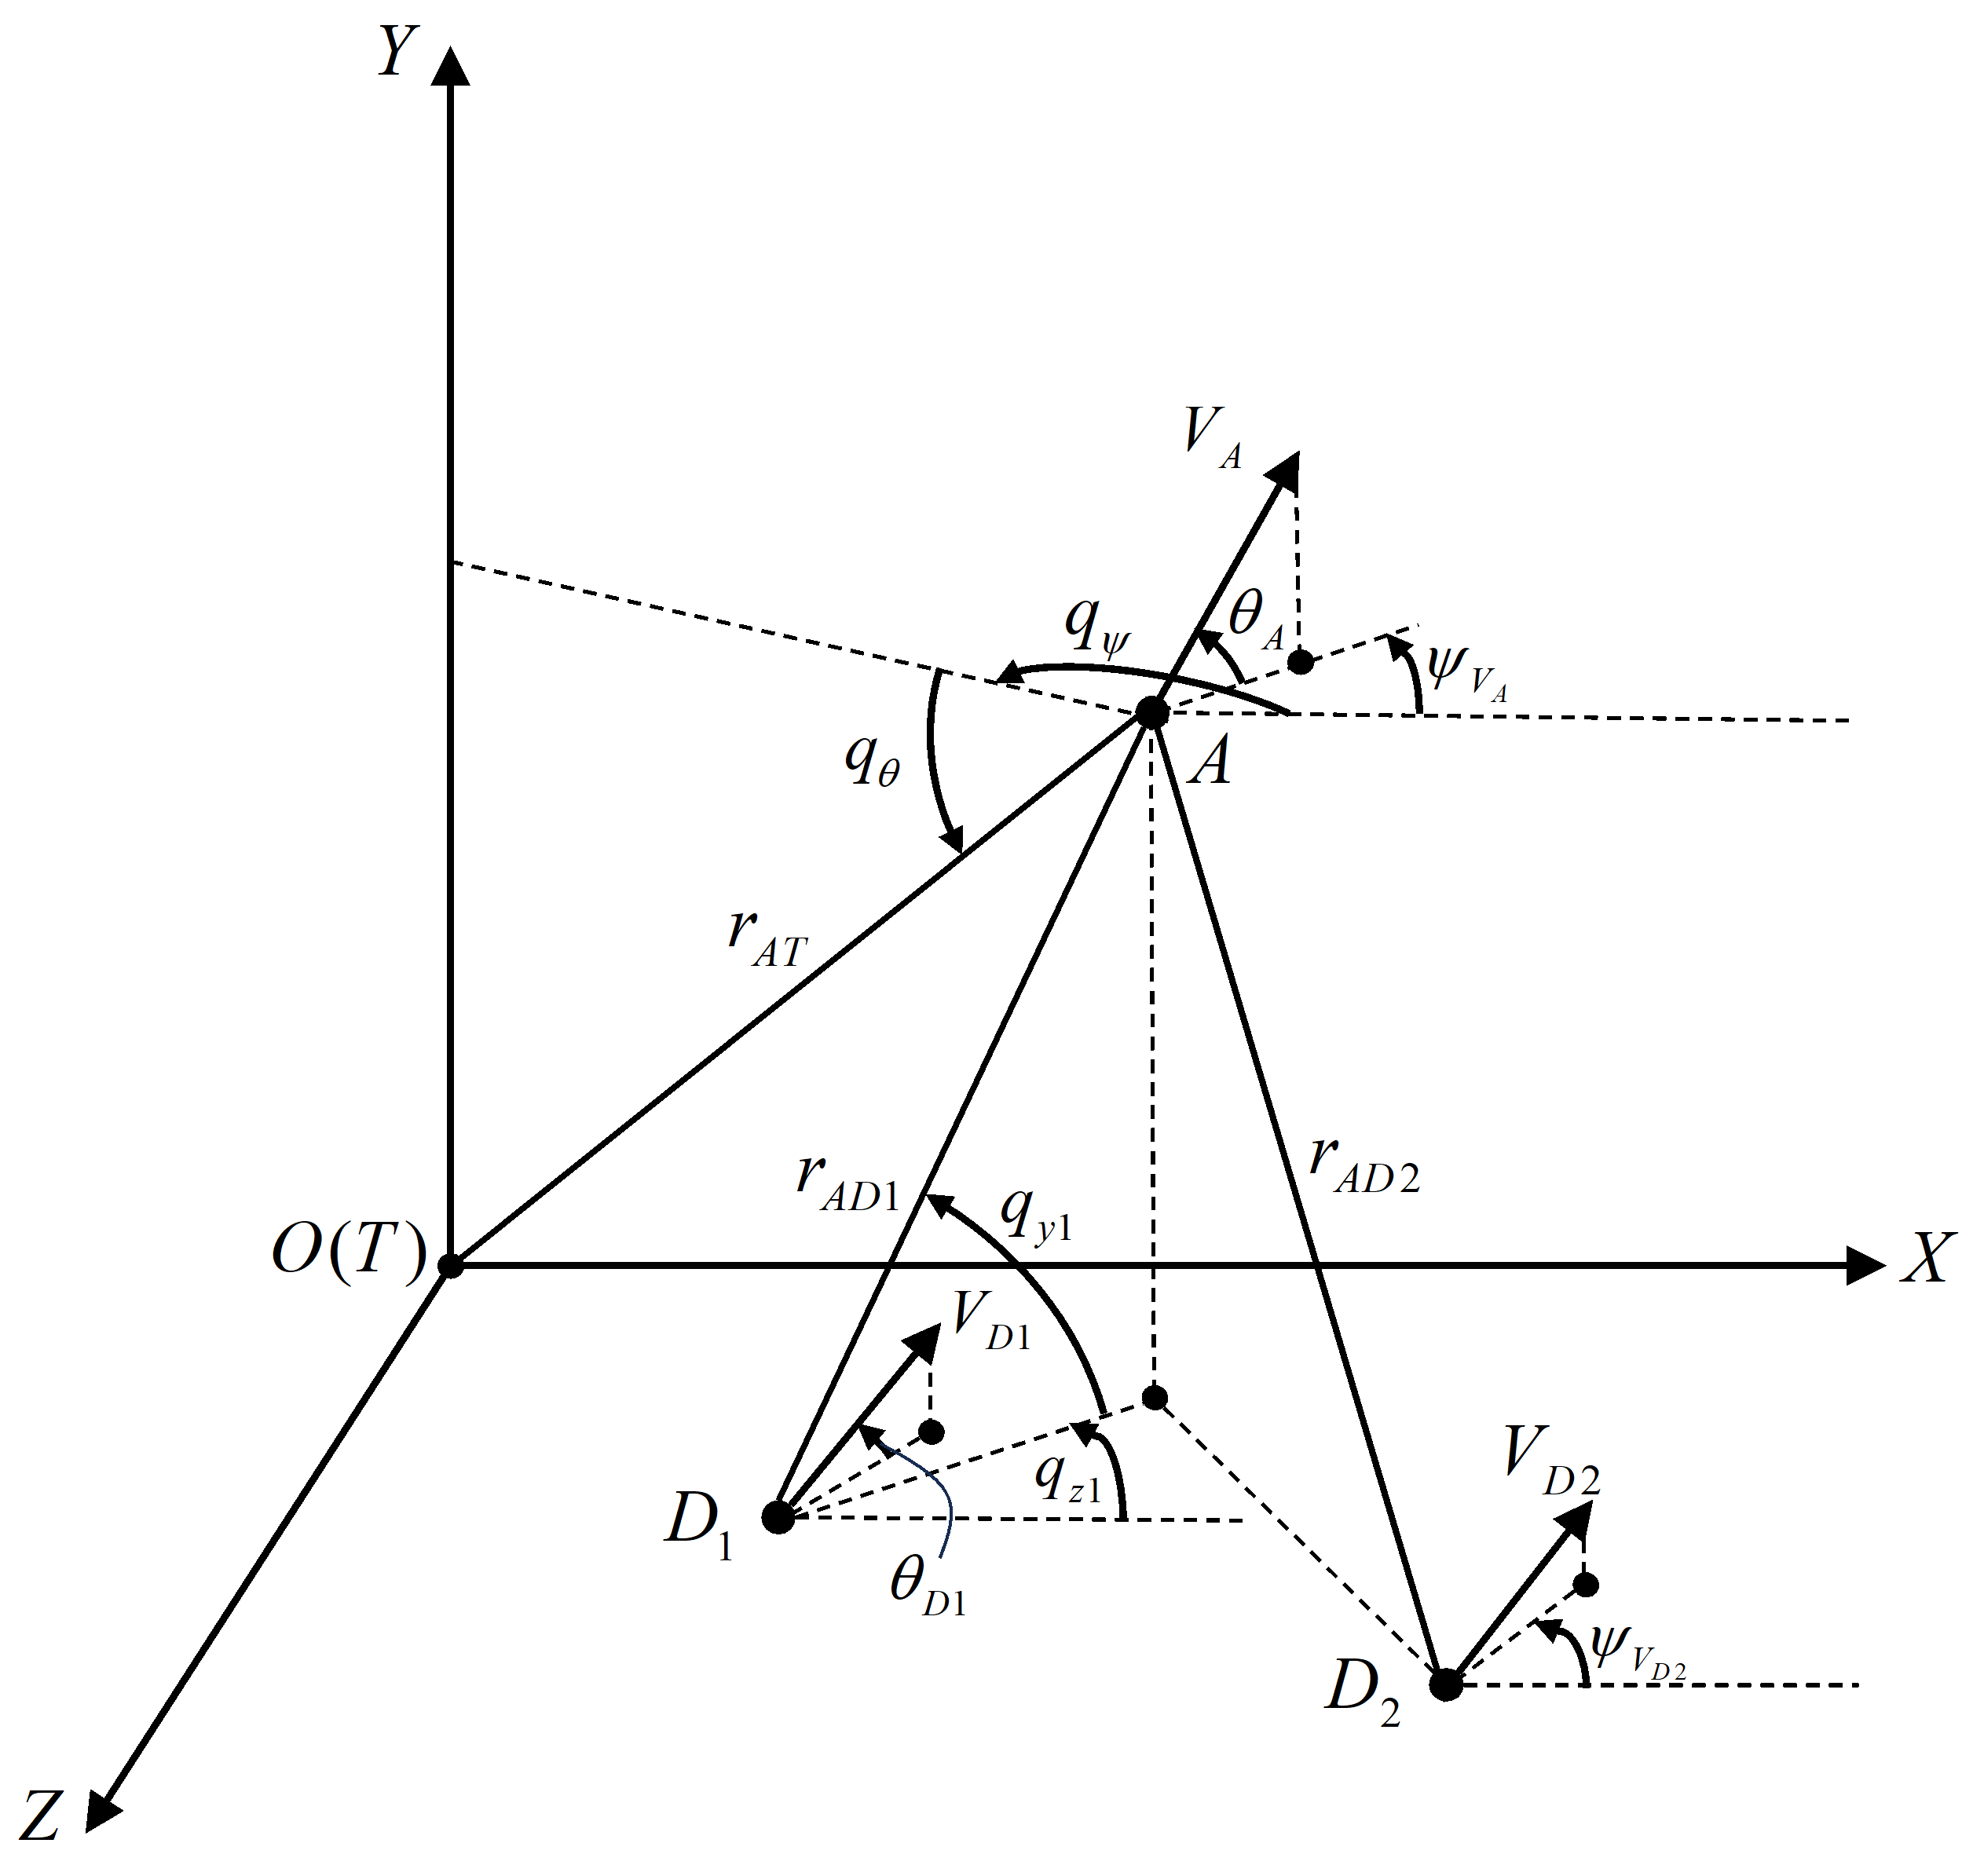
\includegraphics[width=0.585\linewidth]{fig01}
\caption{规避者-目标-NCV 1-NCV 2四体相对运动关系图}
\label{fig:fourbody}
\end{figure}
图~\ref{fig:fourbody}中相对位置和运动关系符号如下表~\ref{tab:symbols}所示。

\begin{table}[!ht]
\centering
\caption{图~\ref{fig:fourbody}相对位置与运动关系符号表}
\label{tab:symbols}
\small
\begin{tabularx}{\linewidth}{lXX}
\toprule
符号 & 含义 & 图~\ref{fig:fourbody}中对应正负 \\
\midrule
${r_{AT}},{r_{ADi}}$ & 规避者与目标、第i枚NCV之间的距离 & 正，正 \\
${q_{yi}},{q_{zi}}$ & 第i枚NCV的俯仰、偏航方向视线角 & 正，正 \\
${q_\theta },{q_\psi }$ & 规避者与目标的俯仰、偏航方向视线角 & 负，正 \\
${V_{Di}},{\theta _{Di}},{\psi _{{V_{Di}}}}$ & 第i枚NCV的速度、航迹倾角和航迹偏角 & 正，正 \\
${V_A},{\theta _A},{\psi _{{V_A}}}$ & 规避者的速度、航迹倾角和航迹偏角 & 正，正 \\
\bottomrule
\end{tabularx}
\end{table}
\FloatBarrier
NCV ${D_1}$, ${D_2}$与规避者$A$的相对运动方程

\begin{equation}
\label{eq:1}
\left\{ {\begin{array}{*{20}{l}}
  \begin{aligned}
& {{\dot r}_{ADi}} =  - {V_{Di}}\left[ {\cos {\theta _{Di}}\cos {q_{yi}}\cos \left( {{q_{zi}} - {\psi _{{V_{Di}}}}} \right) + \sin {\theta _{Di}}\sin {q_{yi}}} \right] +  \\
& {\text{   }}{V_A}\left[ {\cos {\theta _A}\cos {q_{yi}}\cos \left( {{q_{zi}} - {\psi _{{V_A}}}} \right) + \sin {\theta _A}\sin {q_{yi}}} \right]
\end{aligned} \\
  \begin{aligned}
& {{\dot q}_{yi}}{r_{ADi}} = {V_{Di}}\left[ {\cos {\theta _{Di}}\sin {q_{yi}}\cos \left( {{q_{zi}} - {\psi _{{V_{Di}}}}} \right) - \sin {\theta _{Di}}\cos {q_{yi}}} \right] -  \\
& {V_A}\left[ {\cos {\theta _A}\sin {q_{yi}}\cos \left( {{q_{zi}} - {\psi _{{V_A}}}} \right) - \sin {\theta _A}\cos {q_{yi}}} \right]
\end{aligned} \\
  \begin{aligned}
& {{\dot q}_{zi}}{r_{ADi}}\cos {q_{yi}} = {V_{Di}}\cos {\theta _{Di}}\sin \left( {{q_{zi}} - {\psi _{{V_{Di}}}}} \right) -  \\
& {\text{           }}{V_A}\cos {\theta _A}\sin \left( {{q_{zi}} - {\psi _{{V_A}}}} \right)
\end{aligned}
\end{array}} \right.
\end{equation}
规避者和目标相对运动方程

\begin{equation}
\label{eq:2}
\left\{ {\begin{array}{*{20}{l}}
  {{{\dot r}_{AT}} =  - {V_A}\left[ {\sin {q_\theta }\sin {\theta _A} + \cos \left( {{q_\psi } - {\psi _{{V_A}}}} \right)\cos {q_\theta }\cos {\theta _A}} \right]} \\ 
  {{{\dot q}_\theta } = \frac{{{V_A}\left[ {\cos {\theta _A}\sin {q_\theta }\cos \left( {{q_\psi } - {\psi _{{V_A}}}} \right) - \sin {\theta _A}\cos {q_\theta }} \right]}}{{{r_{AT}}}}} \\ 
  {{{\dot q}_\psi } = \frac{{{V_A}\cos {\theta _A}\sin \left( {{q_\psi } - {\psi _{{V_A}}}} \right)}}{{{r_{AT}}\cos {q_\theta }}}} 
\end{array}} \right.
\end{equation}
由运动学关系可得NCV与规避者视线方向相对加速度

\begin{equation}
\label{eq:3}
{\ddot r_{ADi}} = {r_{ADi}}\dot q_{yi}^2 + {r_{ADi}}\dot q_{zi}^2{\cos ^2}{q_{yi}} + {u_{ri}} - {v_{ri}}
\end{equation}
式中，${u_{ri}},{v_{ri}}$分别为规避者和第i枚NCV的加速度在NCV与规避者视线坐标系（设为视线坐标系${S_i}$）x轴投影，坐标系x轴正向定义为NCV指向规避者。

目标与规避者视线方向相对加速度

\begin{equation}
\label{eq:4}
{\ddot r_{AT}} = {r_{AT}}\dot q_\theta ^2 + {r_{AT}}\dot q_\psi ^2{\cos ^2}{q_\theta } + {u_{rT}}
\end{equation}
式中，${u_{rT}}$为规避者加速度在目标与规避者视线坐标系（设为视线坐标系${S_T}$）x轴投影，坐标系x轴正向定义为目标指向规避者。

对每个飞行器，三维运动学方程为:

\begin{equation}
\label{eq:5}
\left\{ {\begin{array}{*{20}{l}}
  {{{\dot x}_j} = {V_j}\cos {\theta _j}\cos {\psi _{{V_j}}}} \\ 
  {{{\dot y}_j} = {V_j}\sin {\theta _j}} \\ 
  {{{\dot z}_j} =  - {V_j}\cos {\theta _j}\sin {\psi _{{V_j}}}} \\ 
  {{{\dot \theta }_j} = \frac{{{a_{yj}}}}{{{V_j}}}} \\ 
  {{{\dot \psi }_j} =  - \frac{{{a_{zj}}}}{{{V_j}\cos {\theta _j}}}} 
\end{array},j = A,{D_1},{D_2}} \right.
\end{equation}
式中，$({x_j},{y_j},{z_j})$为飞行器在地面坐标系位置坐标；${a_{yj}}$, ${a_{zj}}$均垂直于速度矢量，分别表示航迹坐标系$y$、$z$轴上的法向加速度分量，前者位于速度矢量所在铅垂面，后者位于地面系$xOz$水平面内。

由视线方向相对加速度关系式可知，规避者与第i枚NCV的加速度在视线坐标系${S_i}$的x轴投影${u_{ri}}$和${v_{ri}}$，与各自法向加速度${a_{yA}}$,${a_{zA}}$和${a_{yDi}}$,${a_{zDi}}$存在坐标转换关系。设地面坐标系到视线坐标系${S_i}$的转换矩阵为${\mathbf{L}}({q_{yi}},{q_{zi}})$，地面坐标系到航迹坐标系的转换矩阵为${\mathbf{L}}(\theta ,{\psi _V})$，则两者的投影关系可表示为

\begin{equation}
\label{eq:6}
{u_{ri}} = \left[ {\begin{array}{*{20}{c}}
  1&0&0 
\end{array}} \right]{\mathbf{L}}({q_{yi}},{q_{zi}}){{\mathbf{L}}^{ - 1}}({\theta _A},{\psi _{{V_A}}})\left[ {\begin{array}{*{20}{c}}
  0 \\ 
  {{a_{yA}}} \\ 
  {{a_{zA}}} 
\end{array}} \right]
\end{equation}
\begin{equation}
\label{eq:7}
{v_{ri}} = \left[ {\begin{array}{*{20}{c}}
  1&0&0 
\end{array}} \right]{\mathbf{L}}({q_{yi}},{q_{zi}}){{\mathbf{L}}^{ - 1}}({\theta _{Di}},{\psi _{{V_{Di}}}})\left[ {\begin{array}{*{20}{c}}
  0 \\ 
  {{a_{yDi}}} \\ 
  {{a_{zDi}}} 
\end{array}} \right]
\end{equation}
其中转换矩阵的具体形式与三维空间坐标系转换的通用定义一致，此处不再赘述。同理，设地面坐标系到视线坐标系${S_T}$的转换矩阵为${\mathbf{L}}( - {q_\theta },{q_\psi } - \pi )$，其中视线角取${S_T}$的$x$轴正向（目标指向规避者）对应的俯仰、偏航角，则规避者加速度在坐标系${S_T}$的x轴投影

\begin{equation}
\label{eq:8}
{u_{rT}} = \left[ {\begin{array}{*{20}{c}}
  1&0&0 
\end{array}} \right]{\mathbf{L}}( - {q_\theta },{q_\psi } - \pi ){{\mathbf{L}}^{ - 1}}({\theta _A},{\psi _{{V_A}}})\left[ {\begin{array}{*{20}{c}}
  0 \\ 
  {{a_{yA}}} \\ 
  {{a_{zA}}} 
\end{array}} \right]
\end{equation}
\begin{assumption}[NCV制导律与性能]
\label{asm:ncv}
两枚NCV的制导律及性能参数为规避者已知。NCV均采用经典比例导引（PN）制导律\cite{murtaugh1966}，其加速度指令为
\begin{equation}
\label{eq:9}
\left[ {\begin{array}{*{20}{c}}
  {{a_{yDi}}} \\ 
  {{a_{zDi}}} 
\end{array}} \right] = \left[ {\begin{array}{*{20}{c}}
  {{K_{Di}}{V_{Di}}{{\dot q}_{yi}}} \\ 
  { - {K_{Di}}{V_{Di}}{{\dot q}_{zi}}\cos {\theta _{Di}}} 
\end{array}} \right]
\end{equation}
式中，${K_{Di}}$为第i枚NCV比例导引系数。两枚NCV性能相同，即${K_{{D_1}}} = {K_{{D_2}}} = {K_D}$、${V_{{D_1}}} = {V_{{D_2}}} = {V_D}$，其中${K_D}$与${V_D}$在交会过程中保持恒定。
\end{assumption}
两枚NCV的期望规避距离取为相同值，即$d_1^* = d_2^* = d^*$。
\subsection{线性化状态空间模型}
将式\eqref{eq:6}、\eqref{eq:7}及其中的转换矩阵代入式\eqref{eq:3}得

\begin{equation}
\label{eq:10}
\begin{gathered}
  {{\ddot r}_{ADi}} = {r_{ADi}}\left( {\dot q_{yi}^2 + \dot q_{zi}^2{{\cos }^2}{q_{yi}}} \right) - \cos {q_{yi}}\sin \left( {{q_{zi}} - {\psi _{{V_A}}}} \right){a_{zA}} +  \\ 
  {a_{yA}}\left[ { - \cos {q_{yi}}\sin {\theta _A}\cos \left( {{q_{zi}} - {\psi _{{V_A}}}} \right) + \sin {q_{yi}}\cos {\theta _A}} \right] -  \\ 
  {a_{yDi}}\left[ { - \cos {q_{yi}}\sin {\theta _{Di}}\cos \left( {{q_{zi}} - {\psi _{{V_{Di}}}}} \right) + \sin {q_{yi}}\cos {\theta _{Di}}} \right] +  \\ 
  \cos {q_{yi}}\sin \left( {{q_{zi}} - {\psi _{{V_{Di}}}}} \right){a_{zDi}} \\ 
\end{gathered}
\end{equation}
同理，将式\eqref{eq:8}及其中的转换矩阵代入式\eqref{eq:4}得

\begin{equation}
\label{eq:11}
\begin{gathered}
  {{\ddot r}_{AT}} = {r_{AT}}\left( {\dot q_\theta ^2 + \dot q_\psi ^2{{\cos }^2}{q_\theta }} \right) + \left[ {\sin {\theta _A}\cos {q_\theta }\cos \left( {{q_\psi } - {\psi _{{V_A}}}} \right) - \cos {\theta _A}\sin {q_\theta }} \right]{a_{yA}} +  \\ 
  \cos {q_\theta }\sin \left( {{q_\psi } - {\psi _{{V_A}}}} \right){a_{zA}} \\ 
\end{gathered}
\end{equation}
定义状态变量${x_i} = {\left[ {\begin{array}{*{20}{c}}
  {{r_{ADi}}}&{{{\dot r}_{ADi}}} 
\end{array}} \right]^T}$，控制变量\[{u_A} = {\left[ {\begin{array}{*{20}{c}}
  {{a_{yA}}}&{{a_{zA}}} 
\end{array}} \right]^T}\]，则可得规避者与第i枚NCV交互的状态空间方程

\begin{equation}
\label{eq:12}
\mathop {{x_i}}\limits^. (t) = {{\mathbf{A}}_i}{x_i}(t) + {{\mathbf{B}}_i}{u_A}(t) + {{\mathbf{C}}_i}
\end{equation}
式中，\[{{\mathbf{A}}_i} = \left[ {\begin{array}{*{20}{c}}
  0&1 \\ 
  {\dot q_{yi}^2 + \dot q_{zi}^2{{\cos }^2}{q_{yi}}}&0 
\end{array}} \right]\],${{\mathbf{B}}_i} = \left[ {\begin{array}{*{20}{c}}
  0&0 \\ 
  {{B_{1,i}}}&{{B_{2,i}}} 
\end{array}} \right]$,${{\mathbf{C}}_i} = \left[ {\begin{array}{*{20}{c}}
  0 \\ 
  {{C_{1i}}} 
\end{array}} \right]$，其中

\begin{equation}
\label{eq:13}
\left\{ {\begin{array}{*{20}{l}}
  {{B_{1,i}} = \sin {q_{yi}}\cos {\theta _A} - \cos {q_{yi}}\sin {\theta _A}\cos \left( {{q_{zi}} - {\psi _{{V_A}}}} \right)} \\ 
  {{B_{2,i}} =  - \cos {q_{yi}}\sin \left( {{q_{zi}} - {\psi _{{V_A}}}} \right)} \\ 
  {{C_{1i}} = \cos {q_{yi}}\sin \left( {{q_{zi}} - {\psi _{{V_{Di}}}}} \right){a_{zDi}} + [\cos {q_{yi}}\sin {\theta _{Di}}\cos \left( {{q_{zi}} - {\psi _{{V_{Di}}}}} \right) - \sin {q_{yi}}\cos {\theta _{Di}}]{a_{yDi}}} 
\end{array}} \right.
\end{equation}
定义状态变量${x_{AT}} = {\left[ {\begin{array}{*{20}{c}}
  {{r_{AT}}}&{{{\dot r}_{AT}}} 
\end{array}} \right]^T}$，则可得规避者与目标的相对状态空间方程

\begin{equation}
\label{eq:14}
{\dot x_{AT}}(t) = {{\mathbf{A}}_T}{x_{AT}}(t) + {{\mathbf{B}}_T}{u_A}(t)
\end{equation}
式中，\[{{\mathbf{A}}_T} = \left[ {\begin{array}{*{20}{c}}
  0&1 \\ 
  {\dot q_\theta ^2 + \dot q_\psi ^2{{\cos }^2}{q_\theta }}&0 
\end{array}} \right]\],${{\mathbf{B}}_T} = \left[ {\begin{array}{*{20}{c}}
  0&0 \\ 
  {{B_{1,T}}}&{{B_{2,T}}} 
\end{array}} \right]$，其中

\begin{equation}
\label{eq:15}
\left\{
\begin{aligned}
& {B_{1,T}} = \sin {\theta _A}\cos {q_\theta }\cos \left( {{q_\psi } - {\psi _{{V_A}}}} \right) - \cos {\theta _A}\sin {q_\theta } \\
& {B_{2,T}} = \cos {q_\theta }\sin \left( {{q_\psi } - {\psi _{{V_A}}}} \right)
\end{aligned}
\right.
\end{equation}
\begin{remark}
系统\eqref{eq:12}--\eqref{eq:15}为线性时变系统。为获得解析制导指令，在每个制导周期的预测计算中，各矩阵取当前值并视为常值；下一周期再根据更新后的状态重新计算。该拟冻结系数处理也为第4节的在线参数辨识提供了基础。
\end{remark}
\begin{assumption}[量测条件]
\label{asm:meas-noise}
在实际应用中，式\eqref{eq:13}和\eqref{eq:15}中的矩阵元素由机载寻的头/IMU测量得到，而非由无噪声理想运动学计算。测量得到的视线角、视线角速率与飞行器航迹倾角/航迹偏角均叠加零均值高斯白噪声：
\begin{equation}
\label{eq:16}
\begin{gathered}
  \tilde{q}_{\alpha} = {q_{\alpha}} + {\nu _{q,\alpha }},\quad {\nu _{q,\alpha }}\sim \mathcal{N}(0,\sigma _q^2), \hfill \\
  \tildedot{q}_{\alpha} = \dot{q}_{\alpha} + {\nu _{\dot q,\alpha }},\quad {\nu _{\dot q,\alpha }}\sim \mathcal{N}(0,\sigma _{\dot q}^2), \hfill \\
  \tilde{\theta}_{j} = {\theta _{j}} + {\nu _{\theta ,j}},\quad {\nu _{\theta ,j}}\sim \mathcal{N}(0,\sigma _\theta ^2), \hfill \\
  \tilde{\psi}_{V_{j}} = {\psi _{V_{j}}} + {\nu _{\psi ,j}},\quad {\nu _{\psi ,j}}\sim \mathcal{N}(0,\sigma _\psi ^2), \hfill \\ 
\end{gathered}
\end{equation}
式中，$\alpha  \in \left\{ {{y_i},{z_i},\theta ,\psi } \right\}$分别对应与第 $i$ 枚NCV视线和与目标视线各通道，$j \in \left\{ {A,{D_1},{D_2}} \right\}$。雷达导引头对距离与距离率（多普勒）的量测精度通常高于角度量测，本文据此假定相对距离与距离率为精确值，即$\tilde{r} = r$、$\tildedot{r} = \dot{r}$；相对加速度$\ddot{r}$无法直接量测，须由$r$与$\dot{r}$在线估计。规避者实际施加的法向加速度${a_{yA}}$、${a_{zA}}$为机上已知量。式\eqref{eq:13}与\eqref{eq:15}中的矩阵元素由这些含噪测量构成，直接代入将使误差进入制导指令。第4节据此建立在线参数辨识框架：由相对距离运动学恢复矩阵元素，而不依赖对噪声敏感的解析式\eqref{eq:13}/\eqref{eq:15}。
\end{assumption}

\subsection{最优问题建立}
为降低系统阶次并简化求解，引入零控偏差量（ZEM）$z(t)$。定义规避者与第i枚NCV的零控偏差量

\begin{equation}
\label{eq:17}
{z_i}(t) = \left[ {\begin{array}{*{20}{c}}
  1&0 
\end{array}} \right]\Omega \left( {{t_{fi}},t} \right){x_i}(t)
\end{equation}
式中，状态转移矩阵

\begin{equation}
\label{eq:18}
\Omega \left( {{t_{fi}},t} \right) = {e^{{A_i}\left( {{t_{fi}} - t} \right)}} = \left[ {\begin{array}{*{20}{c}}
  {\cosh ({{\dot Q}_i}{t_{{\text{go,i}}}})}&{\frac{{\sinh ({{\dot Q}_i}{t_{{\text{go,i}}}})}}{{{{\dot Q}_i}}}} \\ 
  {{{\dot Q}_i}\sinh ({{\dot Q}_i}{t_{{\text{go,i}}}})}&{\cosh ({{\dot Q}_i}{t_{{\text{go,i}}}})} 
\end{array}} \right]
\end{equation}
其中，${\dot Q_i} = \sqrt {\dot q_{yi}^2 + \dot q_{zi}^2{{\cos }^2}{q_{yi}}} $为视线角速度合成量，${t_{go,i}} = {t_{fi}} - t$为剩余飞行时间。利用状态转移矩阵性质$\dot \Omega \left( {{t_{fi}},t} \right) =  - \Omega \left( {{t_{fi}},t} \right){A_i}$，对式\eqref{eq:17}求导整理可得

\begin{equation}
\label{eq:19}
{\dot z_i}(t) = {\varphi _i}(t)b_i^T{u_A}(t) - {\varphi _i}(t){v_{ri}}
\end{equation}
式中，

\begin{equation}
\label{eq:20}
\left\{
\begin{aligned}
& {\varphi _i}(t) = \frac{{{e^{{{\dot Q}_i}{t_{go,i}}}} - {e^{ - {{\dot Q}_i}{t_{go,i}}}}}}{{2{{\dot Q}_i}}} \\
& {b_i} = {\left[ {\begin{array}{*{20}{c}}
  {{B_{1,i}}}&{{B_{2,i}}}
\end{array}} \right]^T}
\end{aligned}
\right.
\end{equation}
同理可得规避者与目标的零控偏差量导数

\begin{equation}
\label{eq:21}
{\dot z_T}(t) = {\varphi _T}(t)b_T^T{u_A}(t)
\end{equation}
式中，

\begin{equation}
\label{eq:22}
\left\{
\begin{aligned}
& {\varphi _T}(t) = \frac{{{e^{{{\dot Q}_T}{t_{go,T}}}} - {e^{ - {{\dot Q}_T}{t_{go,T}}}}}}{{2{{\dot Q}_T}}} \\
& {b_T} = {\left[ {\begin{array}{*{20}{c}}
  {{B_{1,T}}}&{{B_{2,T}}}
\end{array}} \right]^T}
\end{aligned}
\right.
\end{equation}
其中，${\dot Q_T} = \sqrt {\dot q_\theta ^2 + \dot q_\psi ^2{{\cos }^2}{q_\theta }} $,${t_{go,T}} = {t_{fT}} - t$.

本文智能规避算法的核心目标是在保证成功规避两枚NCV的同时，最小化机动能量消耗，并避免过度机动影响后续目标到达。为此，构建如下二次型性能指标函数

\begin{equation}
\label{eq:23}
\mathop {\min }\limits_{{u_A}} J = \sum\nolimits_{i = 1}^2 {\frac{{{w_i}}}{2}{{\left[ {z_i\left( {{t_{fi}}} \right) - d_i^*} \right]}^2}}  + \frac{{{w_E}}}{2}\int_{{t_0}}^{{t_f}} {u_A^T{u_A}d\tau {\text{ + }}\frac{{{w_T}}}{2}z_T^2\left( {{t_{fT}}} \right)}
\end{equation}
式中，${w_i} > 0$为规避零控偏差量权重，${w_E} > 0$为控制能量权重，${w_T} > 0$为目标到达零控偏差量权重，$d_i^*$为规避者与第i枚NCV的期望规避距离，通常设定为略大于NCV作用半径。${t_f} = \max ({t_{f1}},{t_{f2}})$为全局规避终止时刻。为体现对两枚NCV的均衡规避需求，设${w_1} + {w_2} = w$（$w$为一正常数），且${w_1}$, ${w_2}$满足

\begin{equation}
\label{eq:24}
\left\{
\begin{aligned}
& {w_1} = w \cdot \frac{1}{{1 + {e^{ - \gamma }}}} \\
& {w_2} = w - {w_1} = w \cdot \frac{{{e^{ - \gamma }}}}{{1 + {e^{ - \gamma }}}}
\end{aligned}
\right.
\end{equation}
\begin{problem}[一体化最优规避与制导]
\label{prb:integrated}
考虑\cref{asm:ncv}所述双NCV比例导引交会场景。以规避者法向加速度${u_A} = {[{a_{yA}},{a_{zA}}]^T}$为控制量，在三维四体运动学\eqref{eq:1}--\eqref{eq:5}、状态空间方程\eqref{eq:12}（$i = 1,2$）与\eqref{eq:14}的约束下，并考虑规避者可用最大法向过载给定的指令幅值上限，求最优控制$u_A^*(t)$，使由零控偏差量\eqref{eq:17}与\eqref{eq:21}表述的性能指标\eqref{eq:23}最小，即在两枚NCV各自的交会时刻${t_{f1}}$、${t_{f2}}$将规避零控偏差量驱近期望规避距离$d^*$，在${t_{fT}}$将目标到达零控偏差量驱近零，同时使全程控制能量最小，两项规避权重按式\eqref{eq:24}分配。
\end{problem}

上述问题将规避两枚NCV、到达目标与控制能耗置于同一最优性条件之下，而非分层解耦处理，后文的一体化制导律、制导参数优化与在线参数辨识均围绕其求解展开。

求解\cref{prb:integrated}存在三方面困难。

其一，三项任务由同一控制量耦合，问题不可分解。${u_A}$经投影系数${b_1},{b_2},{b_T}$同时进入三个相对通道，而这些系数随视线几何时变且符号可变：增大与一枚NCV终端间隔的机动可能同时缩小与另一枚的间隔，并改变目标到达通道的零控偏差量；三个终端时刻${t_{f1}},{t_{f2}},{t_{fT}}$互不相同，指示函数还使问题在时间上分段。因此\cref{prb:integrated}既不能退化为两个独立的单NCV规避子问题，也难以在末段有限的剩余飞行时间内依靠在线数值优化求解。第3节据此以极大值原理配合零控偏差量降阶，将上述耦合归结为一个$3 \times 3$线性方程组，从而得到闭环解析制导指令。

其二，性能指标\eqref{eq:23}中的权重无法先验固定。规避权重分配系数$\gamma $与${w_T},{w_E}$的相对大小决定“规避--到达--能量”三者的折中，其最优取值依赖交会几何、剩余飞行时间与可用过载余量：过度偏向规避会使指令长时间贴近过载上限、丧失后续到达能力，过度偏向到达则规避余量不足。故权重选取本身构成沿轨迹求解的非线性优化问题，第5节以打靶法生成的最优专家轨迹预填充经验回放，再由BC-TD3在线给出权重。

其三，解析制导律所需参数在实际量测条件下不可直接获得。${b_i},{b_T}$、${\dot Q_i},{\dot Q_T}$与NCV机动投影${v_{ri}}$均为视线角、视线角速率与航迹角的非线性函数，按\cref{asm:meas-noise}将含噪测量代入解析式\eqref{eq:13}、\eqref{eq:15}会产生有偏且相互相关的误差并直接传入制导指令，相对加速度亦无法直接量测。第4节因此建立带稀疏正则化与遗忘因子的递推最小二乘辨识，由相对距离运动学在线恢复这些参数并与制导律闭环。
